\chapter{Wprowadzenie}
\label{cha:wprowadzenie}


\section{Wstęp}
\label{sec:wstep}

Bezpieczeństwo na drogach stanowi jedno z podstawowych celów postawionych zarówno przez budowniczych dróg, producentów samochodów ich użytkowników a także osób znajdujących się pobliżu. Aby zredukować liczbę wypadków, niezbędne jest uwględnienie ogromnej liczby czynników wpływających na bezpieczeńśtwo na drogach. Należy wziąć pod uwagę warunki atmosferyczne występujące w danej okolicy, ukształtowanie terenu, roślinność która może niekorzystnie wpłynąć na widoczność, drzewa znajdujące się w pobliżu tras oraz samo oznakowanie dróg. Nie należy także lekceważyć statystyk dotyczących wypadków na danych odcinkach dróg. Na bezpieczeństwo na drogach wpływ mają również producenci projazdów. Rozwijane przez nich inteligentne czujniki, systemy wspomagania jazdy mają kluczowe znaczenie w redukcji ryzyka popełnienia błędu przez człowieka.

W tabeli 1.1 znajduje się zestawienie przedstawiające tolerancje biomechaniczną człowieka dla różnych typów pojazdów.

\newcommand{\source}[1]{\caption*{Source: {#1}} }

\begin{table}[ht]
\centering
\caption{Biomechaniczna tolerancha na wypadki}
\label{my-label}
\begin{tabular}{| l | c |}
\hline
\textbf{Typ wypadku}                    & \textbf{Prędkość uderzenia} \\ \hline
samochód / pieszy / rowerzysta          & 20 - 30 km/h                                    \\ \hline
samochód / motocykl                     & 20 - 30 km/h                                    \\ \hline
samochód / drzewo lub słup              & 30 - 40 km/h                                    \\ \hline
samochód / samochód (zderzenie boczne)  & 50 km/h                                         \\ \hline
samochód / samochód (zderzenie czołowe) & 70 km/h   \\ \hline
\end{tabular}
\source{Na podstawie Austroroads 2005}
\end{table}

Z tabeli 1.1 odczytać można, że najbardziej podatni na zagrożenia w ruchu drogowym są piesi, rowerzyści oraz motocykliści. Oczywiście są to uśrednione dane. Ryzyko poważnych obrażeń a nawet śmierci w niektórych przypadkach może dotyczyć przy jeszcze mniejszych prędkośćiach.

\newpage


W ''Raport o stanie bezpieczeństwa ruchu drogowego dla dróg krajowych w zarządzie GDDKiA'' opublikowanym na stronie Generalnej Dyrekcji Dróg Krajowych i Autostrad, znajduje się zestawienie liczby wypadków drogowych i ich skutków, w latach 2007 - 2016.

\begin{figure}[h]
\caption{wypadki drogowe i ich skutki}
\centering
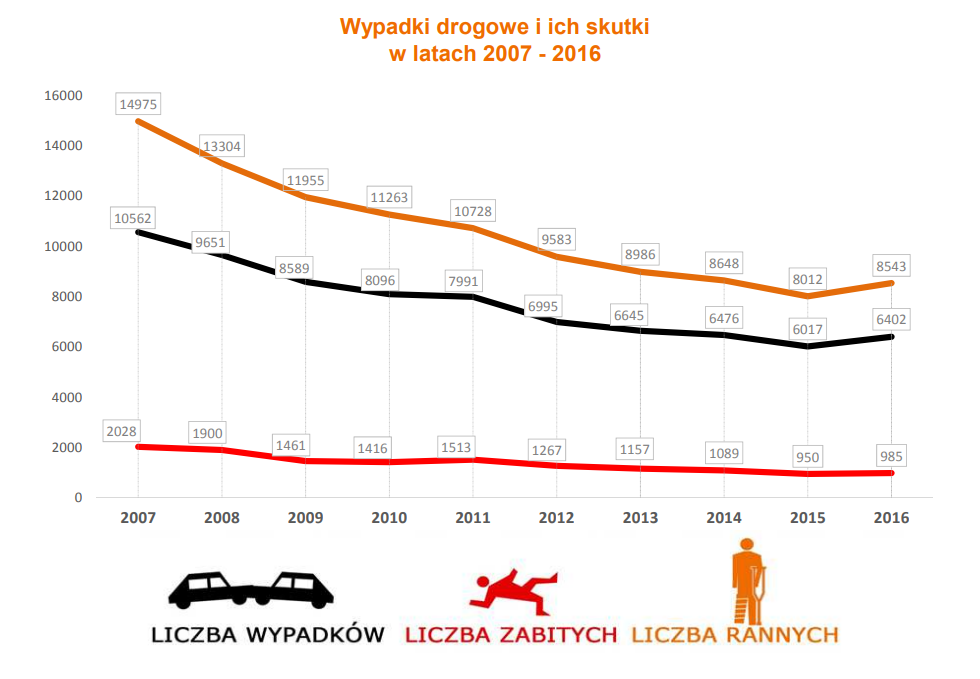
\includegraphics[width=1.1\textwidth]{picture1}
\source{Raport o stanie bezpieczeństwa ruchu drogowego dla dróg krajowych w zarządzie GDDKiA.}
\end{figure}

Z Rys.1.1. odczytać można, że liczba wypadków, z jednym wyjątkiem (z roku 2016) nieustannie maleje. W 2007 roku miało miejsce 10562 wypadków, w których liczba zabitych wyniosła 2028 osób, natomiast rannych było 14975. W porównaniu z 2016 został odnotowany spadek o ok. 40 \%. Niewątpliwie jest to ogromny sukces, jednak liczba ta dalej jest zatrważająco wysoka. 

\newpage
\section{Cele pracy}
\label{sec:celePracy}

Głownym celem niniejszej pracy dyplomowej jest stworzenie inteligentnego systemu, mającego za zadanie predykcję dopuszczalnych prędkości w ruchu drogowym. Ponadto zostaną opracowane modele i narzędzia pozwalające na obliczenie prędkości ma drogach. Rozwiązanie bazować będzie na metodach automatycznego wnioskowania, modelach matematycznych i informacjach geoprzestrzennych. Dzięki temu, możliwe będzie wyznaczenie optymalnego rozwiązania dla złożonego, wielokryterialnego problemu, w którym kluczowe znaczenie będzie miało bezpieczeństwo uczestników ruchu drogowego, przy zachowaniu maksymalnej przepustowości infrastruktury drogowej.

Aglorytm predykcji dopuszczalnych prędkości w ruchu drogowym będzie wykorzystywał następujące informacje

\begin{itemize}
\item \textbf{pojedyńcze poziome zakręty} - zostaną podzielone na trzy grupy, według długości promienia skrętu:
 \begin{itemize}
 	\item \textbf{mały promień skrętu} - o maksymalnej długości promienia 300m
 	\item \textbf{średni promień skrętu} - o długości promienia powyżej 300m i poniżej 600m
 	\item \textbf{duży promień skrętu} - o długości promieniu powyżej 600m 
 \end{itemize}
\item \textbf{połączone poziome zakręty} - będące połączone prostą o długości nie przekraczają 200m. Zostaną podzielone na dwie grupy, według długości promienia skrętu:
 \begin{itemize}
 	\item \textbf{najpierw zakręt o większym promieniu, następnie o mniejszym}
 	\item \textbf{najpierw zakręt o miejszym promieniu, następnie o większym}
 \end{itemize}
\item \textbf{pobliże szkół i miejsc zabaw} - w takich przypadkach prędkość musi zostać dobrana, aby kierowca bez przeszkód mógł zatrzymać się nie powodując zagrożenia dla zdrowia i życia osób niepełnoletnich. Należy mieć na uwadze fakt, że zachowanie małoletnich osób często jest nieobliczalne. Nigdy nie wiadomo kiedy mogą pojawić się na drodze
\item \textbf{pobliże sklepów i miejsc kultów religijnych} - dostosowanie prędkości do większego niż zwykle ruchu pieszych jak i pojazdów mechanicznych.
\item \textbf{pobliże przystanków autobusowych i tramwajowych} - zdażają się szczególne sytuacje, gdy pasażerowie komunikacji zbiorowej, bez patrzenia biegną  do już odjeżdzającej autobusu czy tramwaju. W takim przypadku szczególnie ważne jest dostosowanie prędkości, żeby kierowca mógł bez przeszkód odpowiednio wcześniej zareagować na taką ewentualność
\newpage
\item \textbf{przejścia dla pieszych} - w sytuacjach jak powyżej, z tą różnicą, że zamiast na autobus, przebiegają na "późnym zielonym" lub czasem już czerwonym. Do takich sytuacji najczęściej dochodzi w miastach, gdzie tempo życia jest bardzo duże. Należy pamiętać, że ok. 25\% wypadków na przejściach z sygnalizacją spowodowane jest wtargnięciem pieszego na czerwonym świetle.
\item \textbf{tunele i mosty} - szczególne typy dróg, gdzie w tunelach są inne warunki oświetleniowe, oraz stan nawierzchni w większości przypadków nie jest zależny od warunków atomosferycznych. Mosty zazwyczaj nie są tak szerokie jak ulice do nich prowadzące, dlatego trzeba być przygowanym na np. zwężenia drogi.
\item \textbf{ilość pasów ruchu} - prędkość będzie większa na kilkupasmowej drodze, w porównaniu z jednopasmową
\item \textbf{typ nawierzchni} - jest to bardzo ważny czynnik, ponieważ poruszając się z nieodpowiednią prędkością po nieprzystowowanej do tego nawierzchni, np. żwirowej, bardzo łatwo jest uszkodzić podwozie samochodu
\item \textbf{typ drogi} - autostrady, drogi osiedlowe, eksresowe, główne itp.
\item \textbf{zmiana prędkości między poszczególnymi strefami ograniczeń predkości} - płynna jazda jest znacznie mniej ryzykowna niż nagła zmiana prędkości pojazdu. Dlatego w sytuacjach, gdy na drodzę znajdue np. przejście dla pieszych, należy stopiowo ustawiać coraz to niższe wartości znaków sygnalizującuch ograniczenie prędkości
\item \textbf{przejazdy kolejowe} - są zarówno strzeżone jak i nie strzeżóne. W obu przypadkach należy zachować szczególną ostrożność, dlatego też prędkość musi być odpowiednio niższa. Trzeba mieć na uwadze, że przez dużą masę pojazdów szynowych, wypadki kolejowe należą do jednych z najbardziej śmiercionośnych.
\item \textbf{historia wypadkow} - również jest to dość istotny czynnik, który aglorytm powinien uwględniać
\end{itemize}

Oprócz danych pobranych z OpenStreetMap, apliacja musi posiadać możliwość manualnego - przez zwykłego użytkownika, definiowania obiektów i przeszkód na drodze. Jest to szczególnie istotne, gdyż nie wszystkie dane umieszczone są OSM. 


Kluczową kwestią działanie algorytmu są również miejsce w których powinień umieszczać znaki ograniczenia prędkości. Kierowca odpowiednio wcześniej musi zostać poinformowany o przeszkodzie na drodze, żeby mieć wystarczający czas na reakcję. Dla przykładu, niedopuszczalna jest sytuacja, gdy kierowca podróżując z szybkością 90 km/h, natrafia na znak informujący o znajdującym się za nim przejściu dla pieszych. Prawidłowo działający algorytm, powinień informować o potrzebie stopniowej redukcji prędkości, poprzez umieszczanie znaków ograniczeń prędkości o coraz to mniejszych wartościach. Dzięki temu możliwa będzie płynność jazdy, przy zachowaniu odpowiedniego bezpieczeńśtwa.


%Raport o stanie bezpieczeństwa ruchu drogowego dla dróg krajowych w zarządzenie GDDKiA



\section{Wykorzystane technologie}
\label{sec:wykorzystaneTechnologie}
	Cała aplikacja bazować będzię na dynamicznej stronie internetowej. W tym celu zostanie wykorzystany stos technologiczny, bazujacy na javascripcie, jakim jest MEAN stack. Miałem kilka powodów, dla którym wybrałem te konkretne technologie. Pierwszym jest rosnąca popularność tego stosu. Coraz więcej firm przekonuje sie do tej technologii, więc popyt na programistów z tego zakresu rośnie z roku na rok. Drugim powodem jest fakt, że można go uruchomić na prawie każdym urządzeniu czy platformie, przez co jest duża przenośność kodu. Dodatkowo MEAN stack idealnie nadaje sie do prostych, skalowalnych aplikacji webowych, w których nacisk kładziony jest na intesywną wymianę danych w czasie rzeczywistym na wielu urządzeniach. 
	
	Schemat działania apliacji wygląda następująco. Dane zostaną pobrane z oficjalnej strony OpenStreetMap, 'www.openstreetmap.org'. Są one zapisane w formacie xml. W celu łatwiejszego ich przetwarzania, zostaną przekonwertowane do formatu GeoJson. Jest to rozszerzenia formatu Json o dane niezbędne do operowaniu na geograficznym typie danych. Przetworzone dane, będą przechowywane w mLab. Jest to w pełni zarządzana usługa bazy danych w chmurze, która hostuje bazy danych MongoDB. 

	Back-end aplikacji zostanie napisany w Node.js. Jego głównym zadaniem będzię łączenie się z mLabem w celu pobrania, zapisu, edycji i usuwania danych. Ponadto będzie komunikował się również z frontendem, po to aby przekazywać pobrane dane.  Dodatkowo, w celu zmiejszenia objętości kodu i tym samym zwiekszenia jego czytelności, zostanie użyty framework Express.js. 

	Za zarządzanie front-endem odpowiedzialny będzie angular w wersji 5. Na nim zostanie uruchomiona biblioteka Leaflet. Umożliwia wyświetlenie interaktywnej mapy, którą zasilić będzie można różnymi typami danych, np. w formacie GeoJson. Dzięki niej, użytkownik zyska możliwość wprowadzania swoich danych, przegladania już istniejących czy dowiedzieć sie, jakie prędkości są dozwolone na danych odcinkach dróg. Kolejną, dość istotną funkcjonalnośćią biblioteki leaflet jest możliwość zarządzania wyświetlanymi obiektami. W prosty sposób będzie można ukryć wszystkie dane, wyświetlać tylko drogi, tylko ograniczenia prędkości lub różne kombinację danych, które nas interesują. 
	
\section{Przegląd literatury}
\label{sec:przegladLiteratury}	
	
\section{Układ pracy}
\label{sec:ukladPracy}

Praca składa się z N rozdziałów. 

\begin{itemize}
\item Pierwszy znich zawiera wstęp, cele pracy, wykorzystane technologie oraz przegląd literatury. 
\item Drugi skłąda się z ..., 
\item W trzecim zawarto informacje na temat...
\item Czwarty...
\end{itemize}

